\setboolean{IsHalfPage}{false}%
\setboolean{IsHalfPageLeftCol}{false}%
\setboolean{IsHalfPageRightCol}{false}%
\def\ChapterTitle{%
	Rawa Buntu Station 2.0
}
\def\ChapterUrl{%
	https://arnottferels.github.io/work/rawa-buntu-station-2-0
}
\def\ChapterDescription{%
	Revolutionizing Urban Mobility through `Order in Circulation'
}
\def\ChapterDetailsLine{%
	National Competition -- 2019 | Transit Design; Behavioral Design | South Tangerang, Indonesia
}
\def\ChapterDetailsTabular{%
	\begin{tabular}{@{}ll}
		\textbf{Type}          & National Student Competition by Tarumangara University (Architectural Design Week) \\
		\textbf{Award}         & Top 10                                                                             \\
		\textbf{Contributions} & Research, Conceptual Design, Design Development \& Visualization                   \\
		\textbf{Software}      & SketchUp, Lumion, Photoshop \& Illustrator                                         \\
		\textbf{Collaborators} & Oliver Kenny \& Harry Marvin                                                       \\
		\textbf{URL}           & \textcolor{blue}{\footnotesize\texttt{\href{\ChapterUrl}{\ChapterUrl}}}            \\
	\end{tabular}
}
\def\ChapterAbstract{%
	This project introduces a redesigned station to improve how people move around the existing station. The main idea in this design is called `Order in Circulation.' The key focus is on organizing the movement of passengers, couriers, cars, motorbikes, and apartment residents. By solving the main issues at Rawa Buntu Station, the overall urban environment is expected to become more efficient and organized.
}
\StartTwoColumnLayout
\chapter*{\ChapterTitle}\addcontentsline{toc}{chapter}{\ChapterTitle}
\ChapterSetTocAddData{\ChapterDetailsLine}
\ChapterSetDetailsData{\ChapterDescription}{\ChapterDetailsLine}{\ChapterDetailsTabular}
\RuleAbstract
\ChapterAbstract
\section*{
  Issues \& Strategies
 }
%
\begin{figure}[H]
	\centering
	\includesvg[width=\linewidth]{src/graphics/rawa-buntu-station-2-0--issues-strat.svg}
	\label{
		fig:rawa-buntu-station-2-0--issues-strat
	}
\end{figure}

\vfill
\begin{center}
	\begin{minipage}{0.9\linewidth}
		%
\begin{figure}[H]
	\centering
	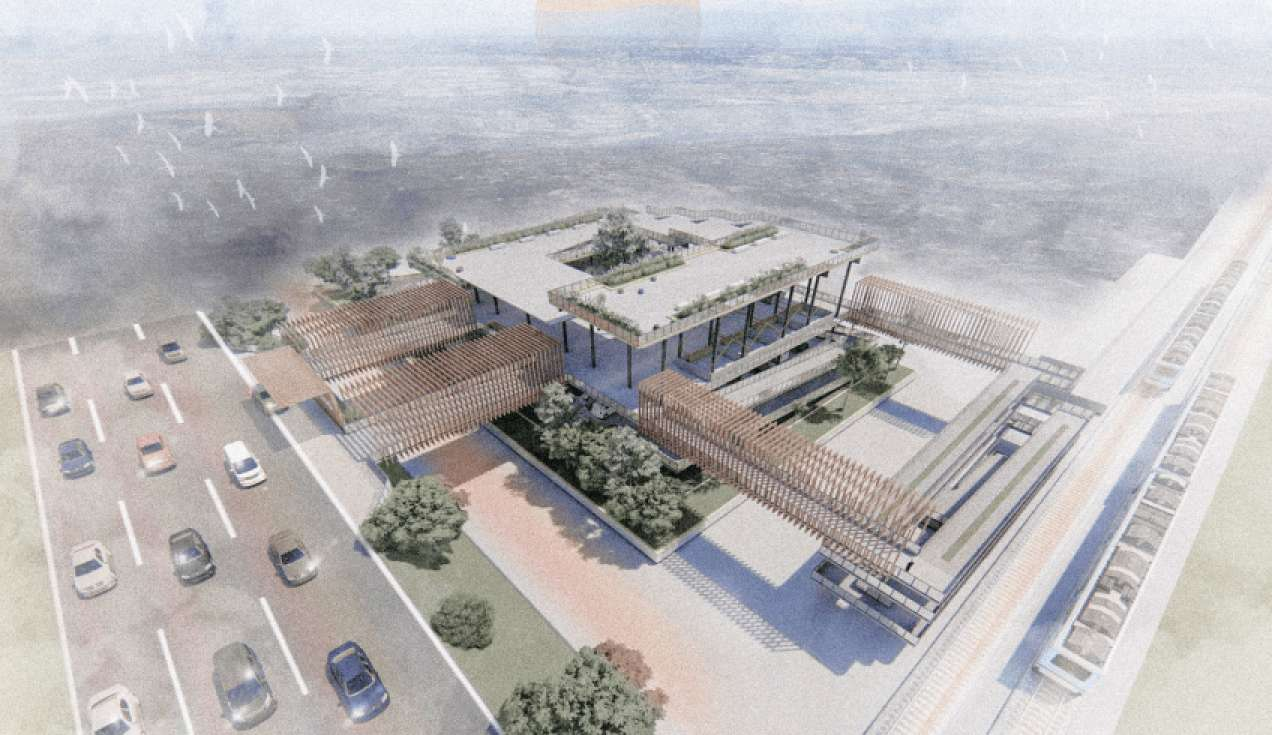
\includegraphics[width=\linewidth]{src/graphics/rawa-buntu-station-2-0--perspective-aerial.jpg}
	\caption*{
		Aerial view -- The bridge \& viewing deck
	}
	\label{
		fig:rawa-buntu-station-2-0--perspective-aerial
	}
\end{figure}

	\end{minipage}
\end{center}
\columnbreak%
\section*{
  Concept \& Programming -- Order in Circulation
 }
%
\begin{figure}[H]
	\centering
	\includesvg[width=\linewidth]{src/graphics/rawa-buntu-station-2-0--concept.svg}
	\label{
		fig:rawa-buntu-station-2-0--concept
	}
\end{figure}

\vfill
This initiative aims to create a distinctive public parking facility by emphasizing comfort, openness, and inclusivity, including features for people with disabilities. The goal is to encourage a shift in community behavior towards utilizing public transportation, reducing the impact of traffic congestion.
\vfill
\begin{center}
	\begin{minipage}[b]{0.875\linewidth}
		\setlength{\columnsep}{0.5cm}
		\begin{multicols}{2}
			%
\begin{figure}[H]
	\centering
	\begin{tikzpicture}
		\node[inner sep=0pt] (Image) at (0,0) {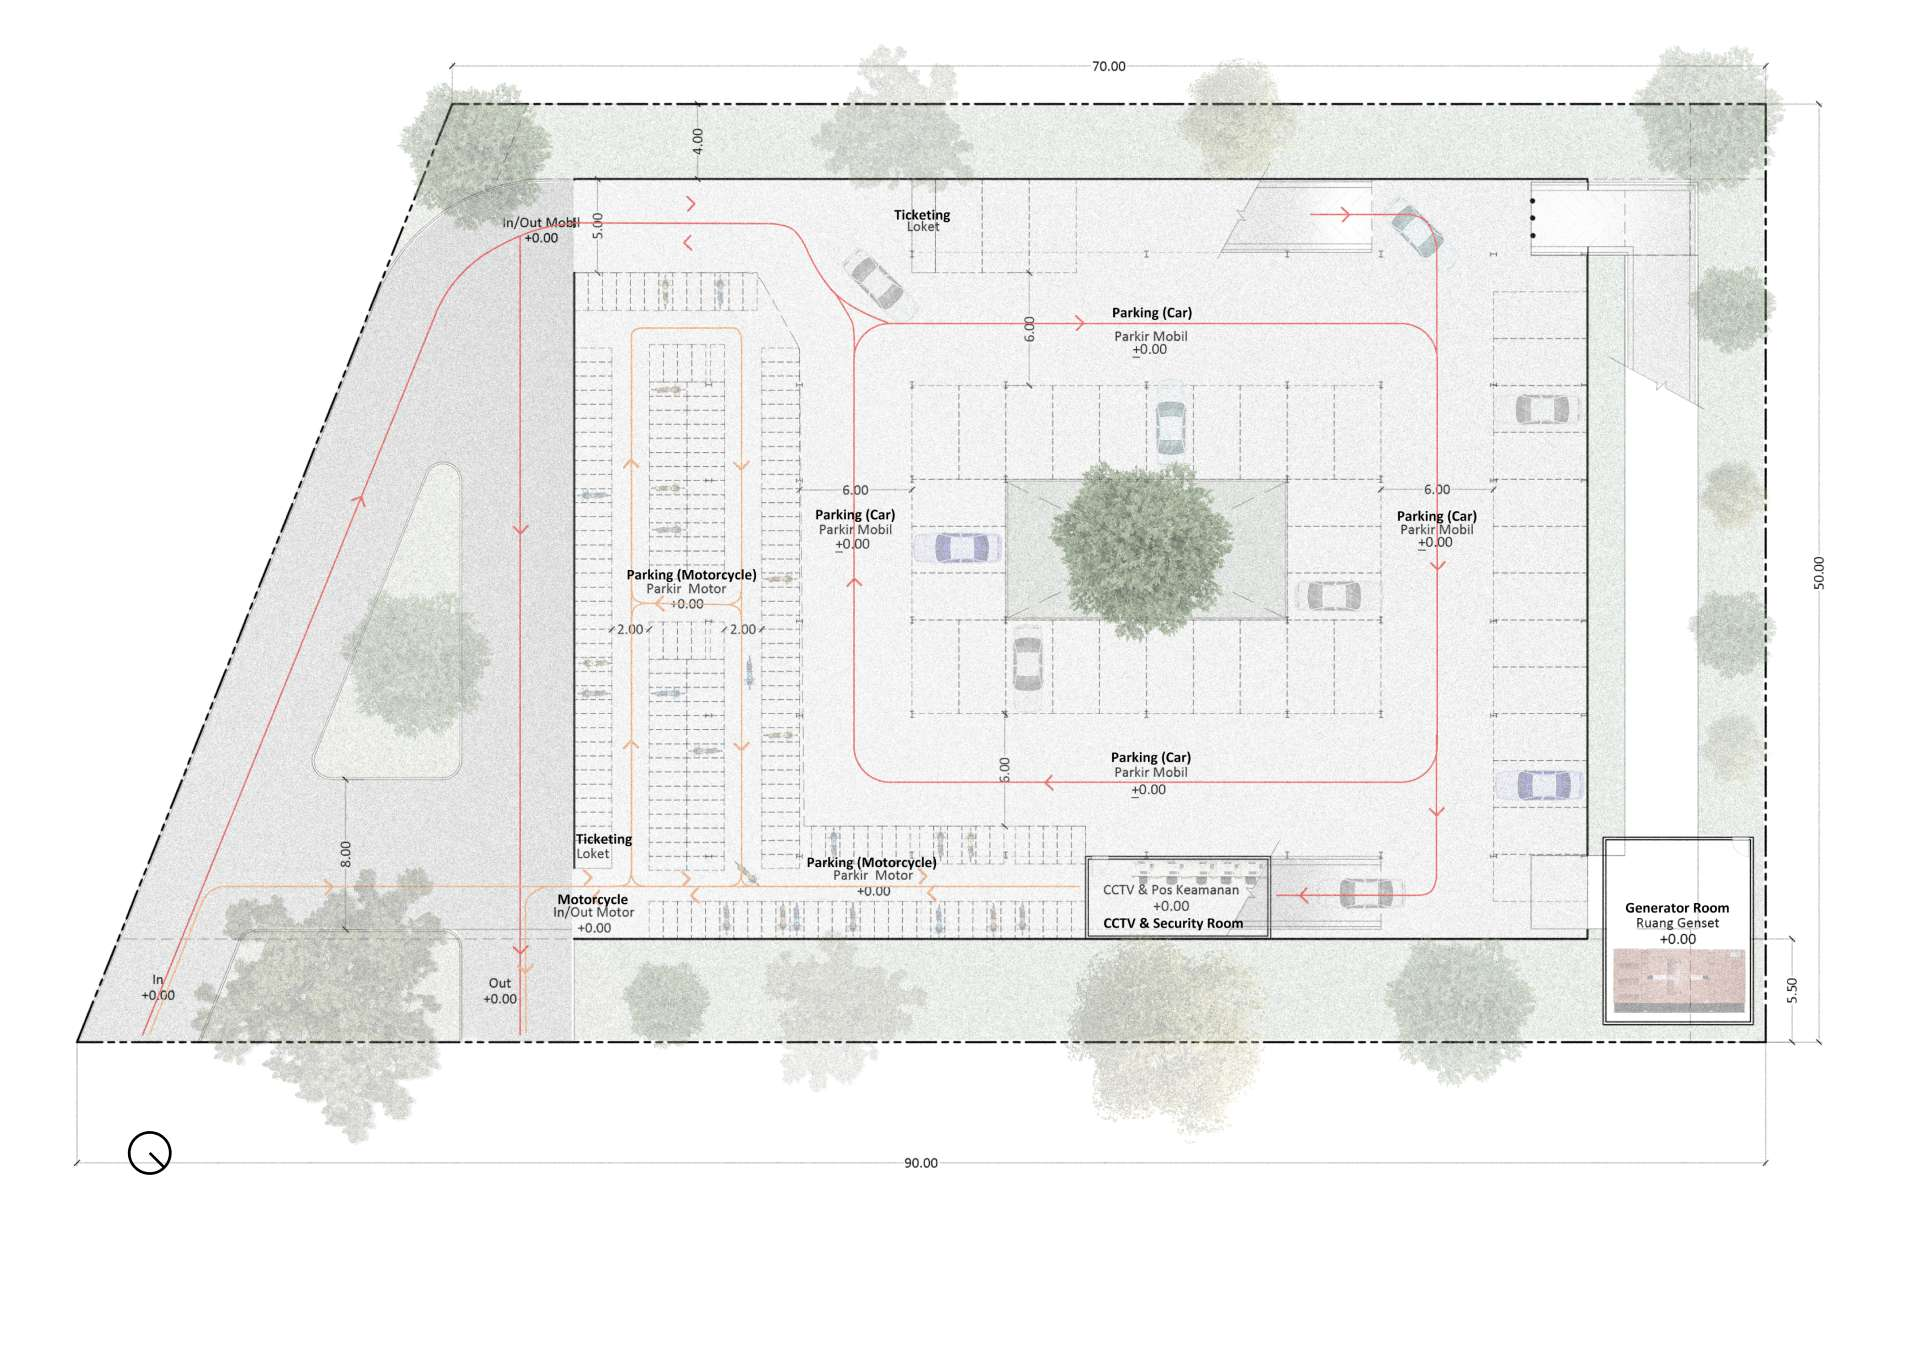
\includegraphics[width=\linewidth, keepaspectratio]{src/graphics/rawa-buntu-station-2-0--level-01.jpg}};
		\node[align=center, text=black, text width=0.75\linewidth, yshift=+6pt] at (Image.south) {\footnotesize \setlength{\baselineskip}{0pt}\selectfont {Level 1}};
	\end{tikzpicture}
	\label{
		fig:rawa-buntu-station-2-0--level-01
	}
\end{figure}

			%
\begin{figure}[H]
	\centering
	\begin{tikzpicture}
		\node[inner sep=0pt] (Image) at (0,0) {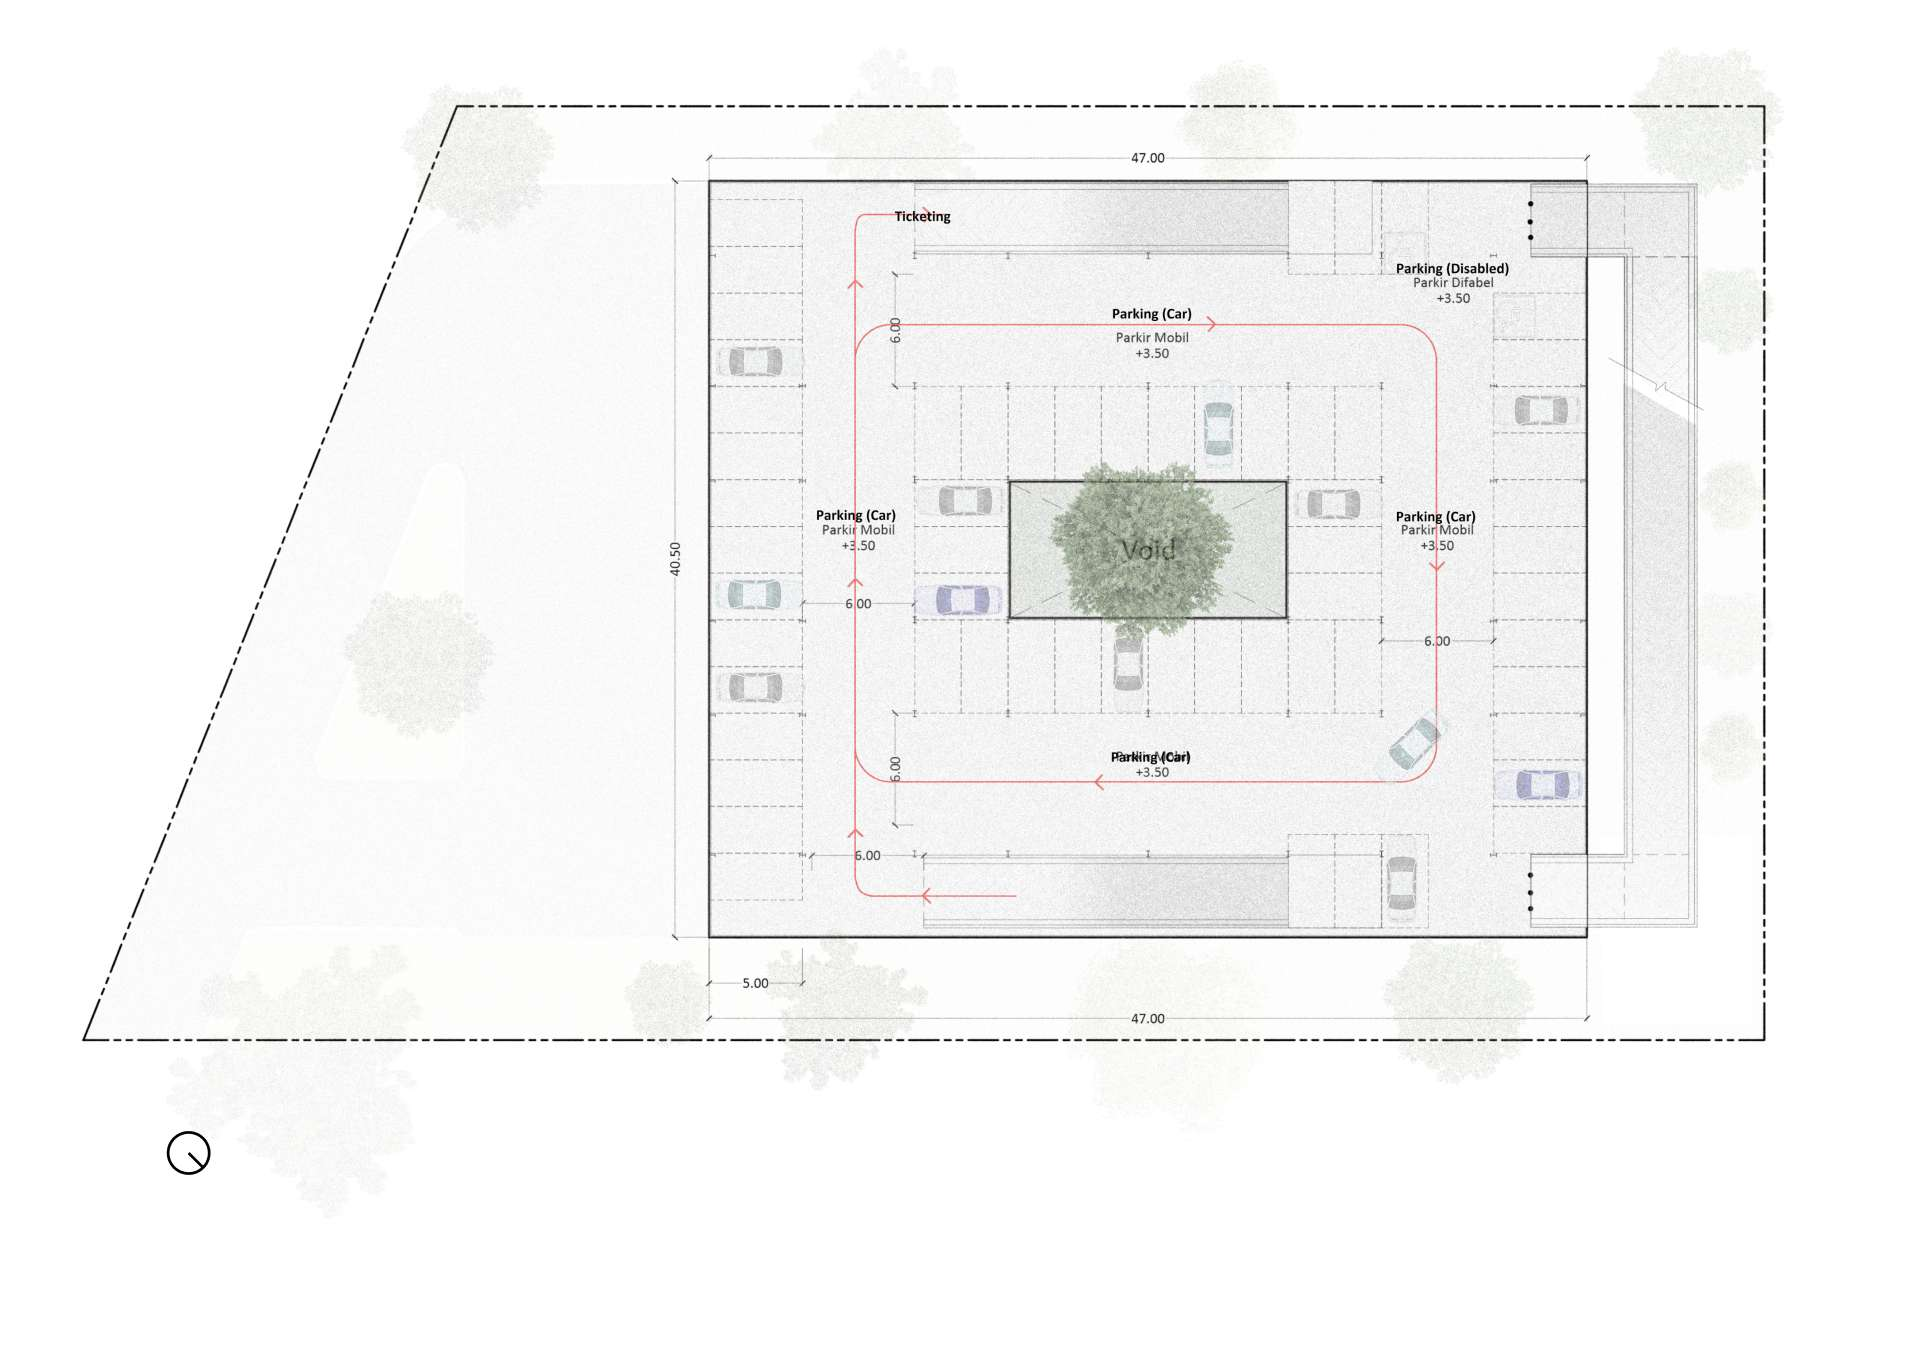
\includegraphics[width=\linewidth, keepaspectratio]{src/graphics/rawa-buntu-station-2-0--level-02.jpg}};
		\node[align=center, text=black, text width=0.75\linewidth, yshift=+6pt] at (Image.south) {\footnotesize \setlength{\baselineskip}{0pt}\selectfont {Level 2}};
	\end{tikzpicture}
	\label{
		fig:rawa-buntu-station-2-0--level-02
	}
\end{figure}

			%
\begin{figure}[H]
	\centering
	\begin{tikzpicture}
		\node[inner sep=0pt] (Image) at (0,0) {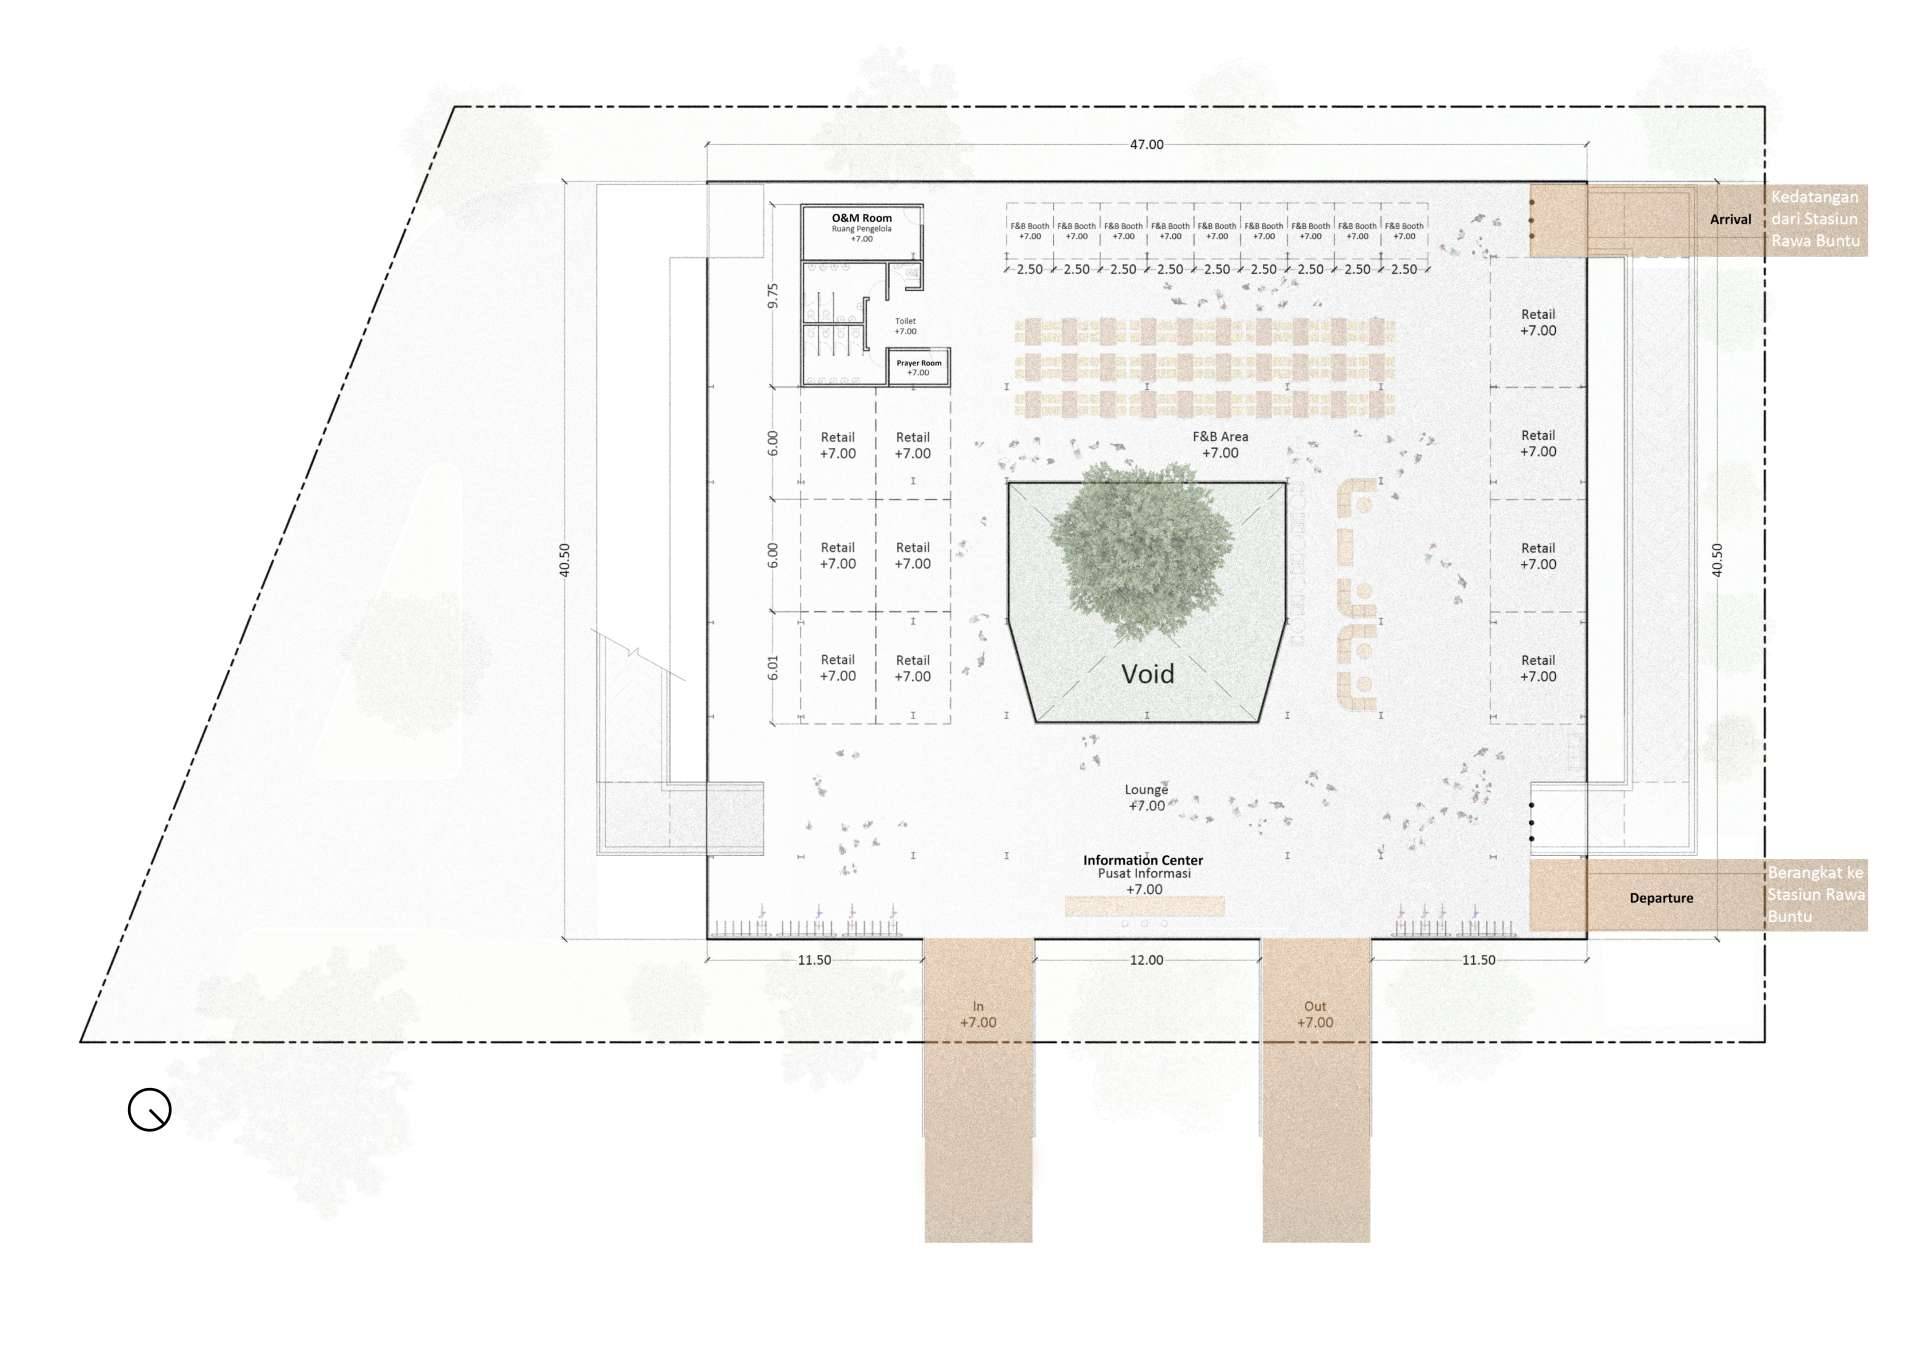
\includegraphics[width=\linewidth, keepaspectratio]{src/graphics/rawa-buntu-station-2-0--level-03.jpg}};
		\node[align=center, text=black, text width=0.75\linewidth, yshift=+6pt] at (Image.south) {\footnotesize \setlength{\baselineskip}{0pt}\selectfont {Level 3}};
	\end{tikzpicture}
	\label{
		fig:rawa-buntu-station-2-0--level-03
	}
\end{figure}

			%
\begin{figure}[H]
	\centering
	\begin{tikzpicture}
		\node[inner sep=0pt] (Image) at (0,0) {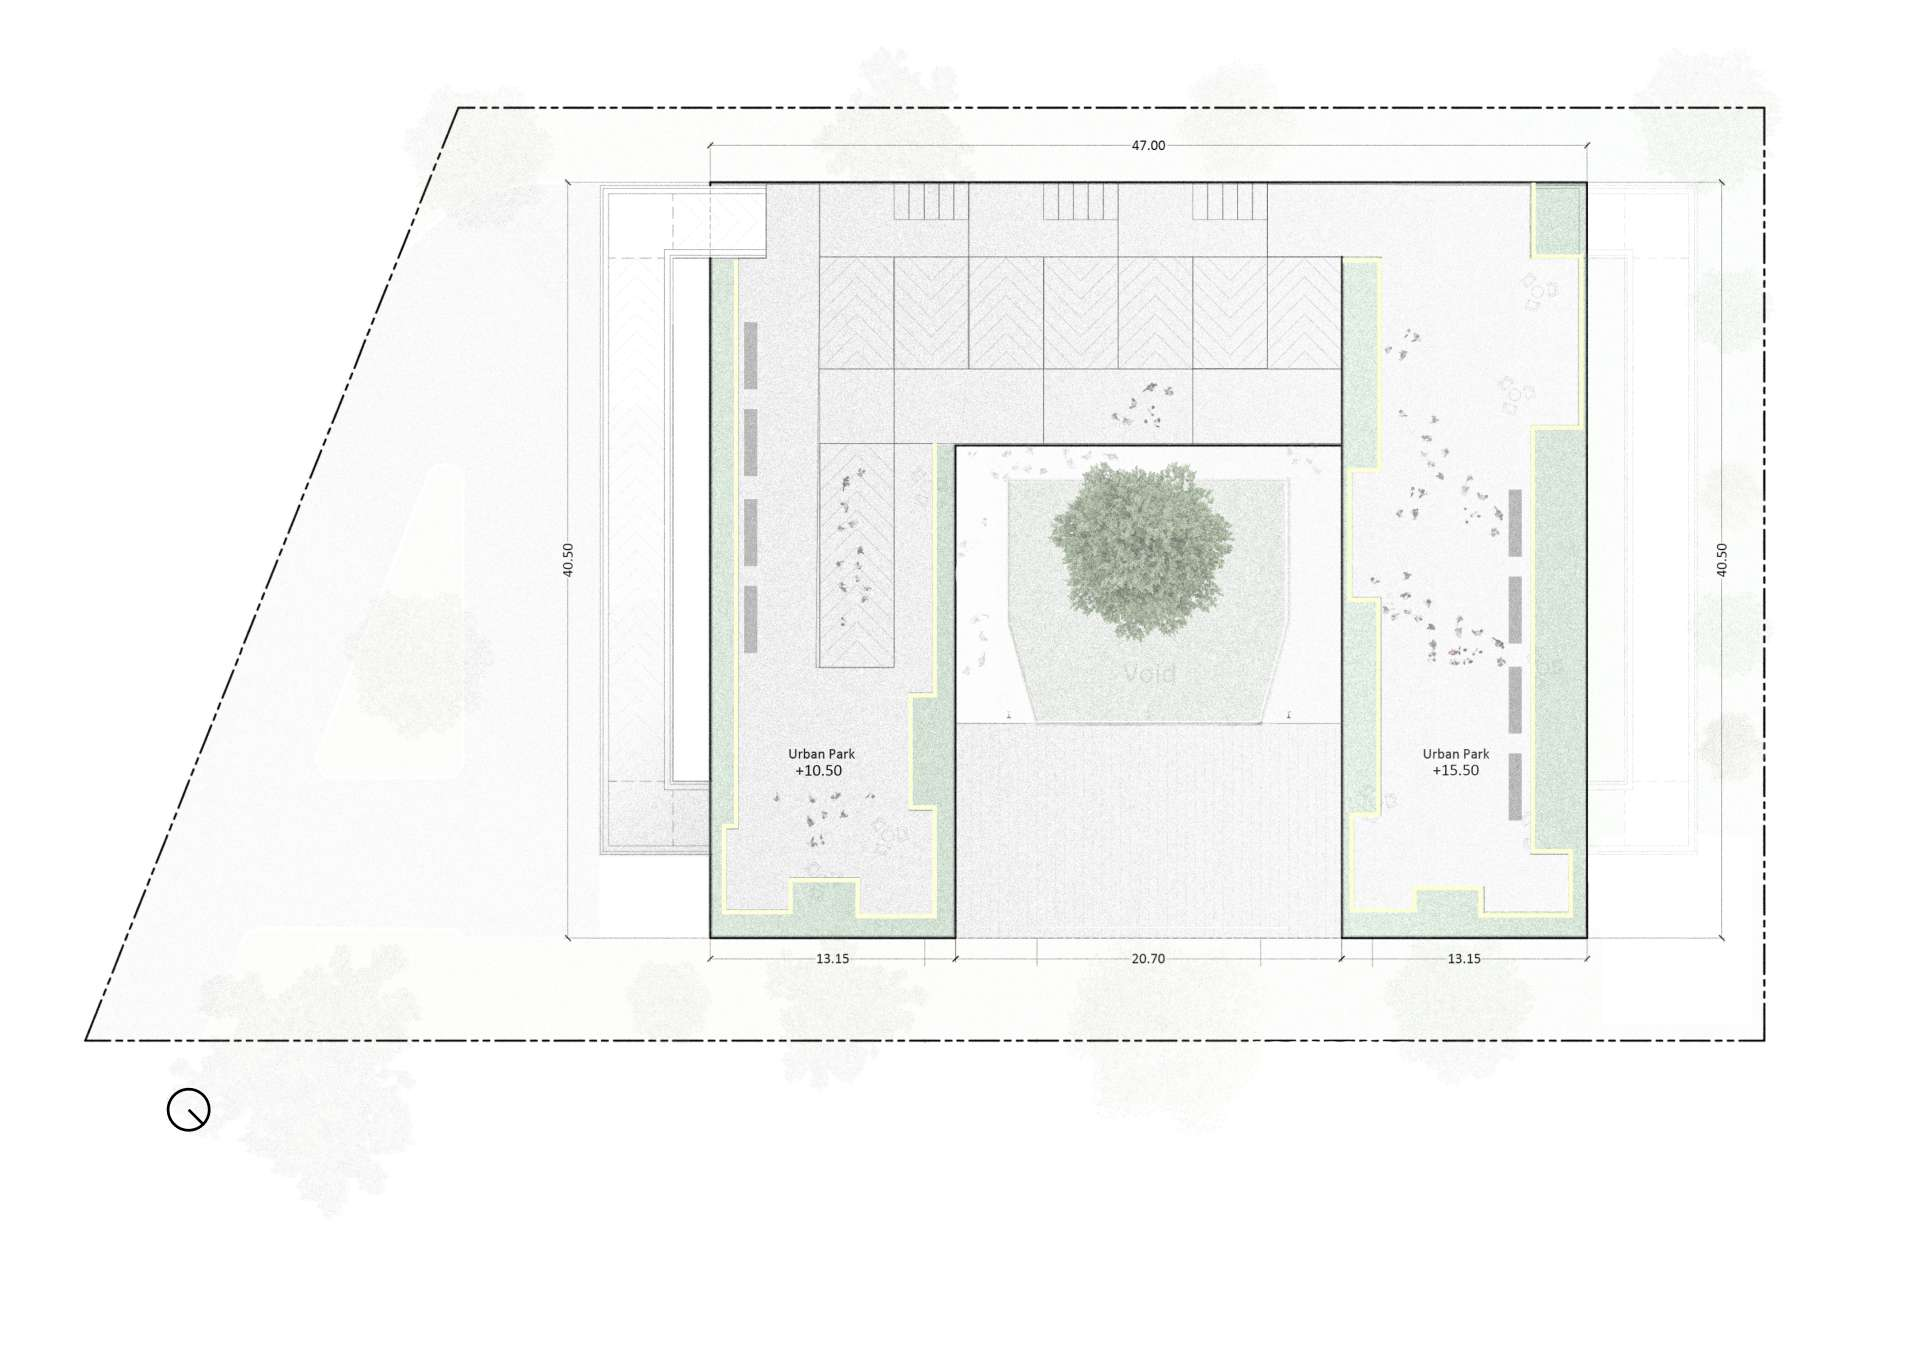
\includegraphics[width=\linewidth, keepaspectratio]{src/graphics/rawa-buntu-station-2-0--level-04-rooftop.jpg}};
		\node[align=center, text=black, text width=0.75\linewidth, yshift=+6pt] at (Image.south) {\footnotesize \setlength{\baselineskip}{0pt}\selectfont {Level 4 (Rooftop)}};
	\end{tikzpicture}
	\label{
		fig:rawa-buntu-station-2-0--level-04-rooftop
	}
\end{figure}

		\end{multicols}
		\vfill
		%
\begin{figure}[H]
	\centering
	\includesvg[width=\linewidth]{src/graphics/rawa-buntu-station-2-0--section.svg}
	\caption*{
		Front elevation (Southwest)%
	}
	\label{
		fig:rawa-buntu-station-2-0--section
	}
\end{figure}

		\vfill
		\setlength{\columnsep}{0.5cm}
		\begin{multicols}{2}
			%
\begin{figure}[H]
	\centering
	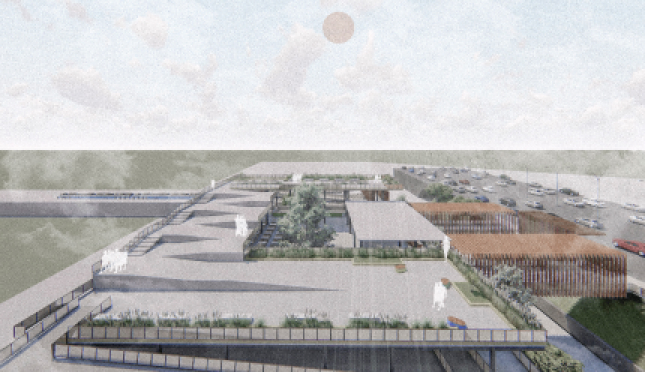
\includegraphics[width=\linewidth]{src/graphics/rawa-buntu-station-2-0--perspective-01.jpg}
	\caption*{
		The Bridge \& viewing deck
	}
	\label{
		fig:rawa-buntu-station-2-0--perspective-01
	}
\end{figure}

			%
\begin{figure}[H]
	\centering
	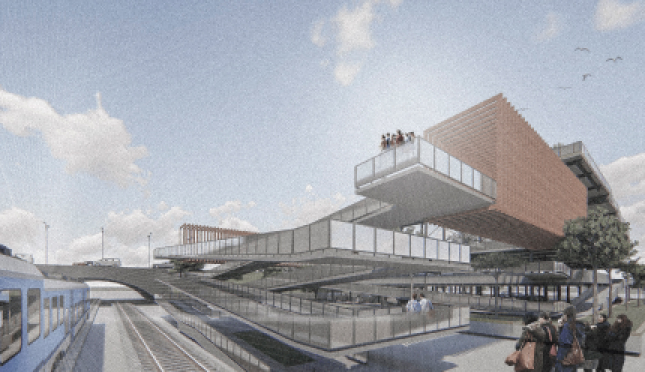
\includegraphics[width=\linewidth]{src/graphics/rawa-buntu-station-2-0--perspective-02.jpg}
	\caption*{
		Ramp from/to the train platform
	}
	\label{
		fig:rawa-buntu-station-2-0--perspective-02
	}
\end{figure}

		\end{multicols}
	\end{minipage}
\end{center}
\EndTwoColumnLayout
\newpage
